\section{Results}

\subsection{Accurate Classification of Breast Neoplasmas in the BreakHis Dataset}

Transfer-learning the VGG16 on the unmodified BreakHis dataset results in acceptable overall classification accuracy (70\%), however closer inspection reveals bias towards one of the classes (ductal carcinoma) due to imbalances in the number of examples between classes (\emph{Figure \ref{fig:confmat}a}). Oversampling the dataset such that all classes have an equal number of training examples resulted in a small improvement in overall classification accuracy (72\%), and shows a demonstrable reduction in bias (\emph{Figure \ref{fig:confmat}b}).\par

Notably, lobular carcinomas were mistaken for ductal carcinomas in just over two-thirds of the validation set, and correctly identified a quarter of lobular carcinoma examples. After oversampling the BreakHis dataset, the accuracy and ductal carcinoma false-positive rates have nearly replaced one another, with lobular carcinomas being correctly classified in 63\% of cases and false ductal carcinoma classifications in a quarter of cases. Ductal carcinoma false-positives were in fact halved, on average, across nearly all classes after oversampling.\par

\begin{figure}[ht!]
	\begin{center}
		\caption{Confusion Matrix of VGG16 Model Trained on the Original and Oversampled BreakHis Datasets \label{fig:confmat}}
	\end{center}
	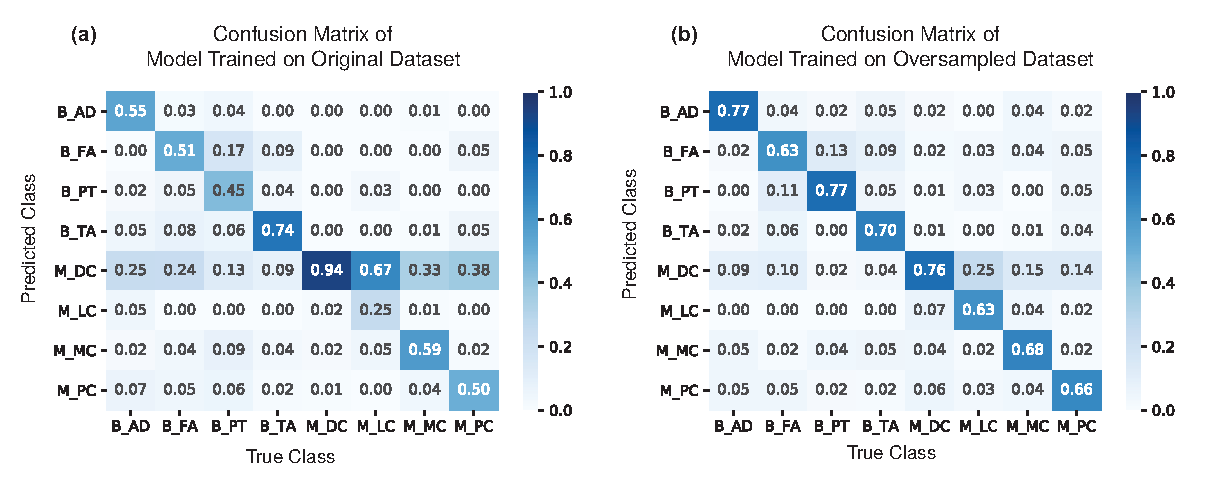
\includegraphics[width=170mm]{figures/deepduct/confusion_matrix.pdf}
	\begin{singlespace}
		\textit{Legend} --- Confusion matrices of the VGG16 model either trained on (a) the original BreakHis dataset as provided by its creators, or (b) a modified version of the BreakHis dataset oversampled such that each class has the same number of training examples. The model trained on the original dataset achieved an average accuracy of 70\% on the validation set across all classes, while the oversampled model saw a modest increase for a final average accuracy of 72\%. See Appendix A for class code legend used in this figure.
	\end{singlespace}
	
\end{figure}